\documentclass{article}
\usepackage[margin=1.1in]{geometry}
\usepackage{graphicx}
\usepackage{caption}
\usepackage{ctable}
\usepackage{booktabs}
\usepackage{fancyhdr}
\usepackage{wrapfig}
\usepackage{float}
\usepackage{caption}
\usepackage{subcaption}
\usepackage{amsmath}
\usepackage{amsfonts}
\usepackage{amssymb}
\usepackage{amsthm}
\usepackage{mathtools}
\usepackage{mathrsfs}
\usepackage{url}

\newcommand\prn[1]{\left( #1 \right)}
\newcommand\bkt[1]{\left[ #1 \right]}
\newcommand\set[1]{\left\{ #1 \right\}}
\newcommand\abs[1]{\left| #1 \right|}

\pagestyle{fancy}
\lhead{\footnotesize \textsc{Natoli}}
\rhead{\footnotesize \thepage}
\cfoot{}
\frenchspacing


\title{\vspace{-20pt}Dynamics of a Heterogeneous Agent-Based Model\\of Financial Markets\thanks{This work made use of the Sullivan supercomputer of the Open Science Data Cloud, which is an Open Cloud Consortium (OCC)-sponsored project. This work was supported in part by grants from Gordon and Betty Moore Foundation and the National Science Foundation and major contributions from OCC members like the University of Chicago.}}
\author{\textit{Author:} Christopher Natoli\\
  \textit{Instructor:} Leonard Smith\\
  University of Chicago\\}
\date{}

\begin{document}

\maketitle

\section{Introduction}

This paper implements and examines a model put forward by J. Doyne Farmer and extended by Rui Carvalho. Farmer's model \cite{farmer} is a simple representation of a financial market in which there is one stock and two heterogeneous types of traders, those who invest based on the fundamental value of the stock (called ``fundamentalists'') and those who follow trends (called ``chartists''). Farmer's model has two key advantages over other financial models: it is not an aggregation based on a single representative agent, and it does not assume that markets clear to achieve an equilibrium price.

Carvalho extends this model by assigning each trader a probability of being active during each trading period \cite{carvalho}. Interestingly, Carvalho's model exhibits leptokurtotic returns, i.e., fat tails and a sharper peak, as well as clustered volatility, i.e., the volatility today tends to be correlated with the volatility yesterday. Both these properties are present in real financial markets but not present in models involving rational expectations and price equilibria.

The model implemented for this paper and discussed by Carvalho is driven by a dialogue between the ``market maker'' and the traders. Every period, the market maker collects the orders from the traders. In the $(t+1)$th period, the $i$th fundamentalist orders $\omega_{t+1}^{(i)}$ amount of the stock according to
$$
\omega_{t+1}^{(i)}=-c^{(i)}\prn{(p_t-p_{t-1})-(v_t-v_{t-1})}
,$$
where $c^{(i)}$ is the $i$th trader's capital, $p_t$ is the log price of the stock at time $t$, and $v_t$ is the log fundamental value of the stock at time $t$. The fundamental value of the stock follows a random walk with normally distributed steps. Notably, the fundamentalists in this model do not care about the difference between the market price $p_t$ and the fundamental value $v_t$. They instead care about how much the market price has grown relative to how much the fundamental price has grown. Farmer argues that the former strategy is unrealistic since it could produce unbounded positions, e.g., if the market price is consistently below the fundamental price, then fundamentalists would buy stock every period.

The $i$th chartist orders
$$
\omega_t^{(i)}=c^{(i)}\prn{r_t-r_{t-\theta^{(i)}}}
,$$
where $r_t=p_t-p_{t-1}$ is the log return in period $t$ and $\theta^{(i)}$ is the lag that the $i$th trader is interested in. I.e., a chartist is interested in how much the market price has grown yesterday relative to how much it had grown $\theta^{(i)}$ periods ago.

Trader $i$ is active in period $(t+1)$ with probability $p^{(i)}$. Define the random variable $\delta^{(i)}_{t+1}$ that is 1 if the trader is active in period $(t+1)$ and 0 otherwise. The market maker then aggregates all these orders and sets the new price according to
$$
p_{t+1}=p_t+\frac{1}{\lambda}\sum\delta_{t+1}^{(i)}\omega_{t+1}^{(i)},
$$
where $\lambda$ is a normalization constant. Every period, the fundamental value takes a random step, and the process repeats.

This system was implemented in an object-oriented framework.\footnote{The code is available at \url{https://github.com/chrisnatoli/agent-based_finance/}.} The particular settings of the system discussed below follow Carvalho: The number of fundamentalists is 5000 and the number of chartists is also 5000. Every trader has a capital $c^{(i)}$ of 0.08 and a probability $p^{(i)}$ of being active of 0.01. The chartists' lags $\theta^{(i)}$ are uniformly distributed integers between 1 and 100 (inclusive). The normalization constant is $\lambda=1$ and the fundamental price follows a random walk with zero drift and standard deviation $0.1$.
\begin{wrapfigure}{r}{0.5\textwidth}
  \centering
  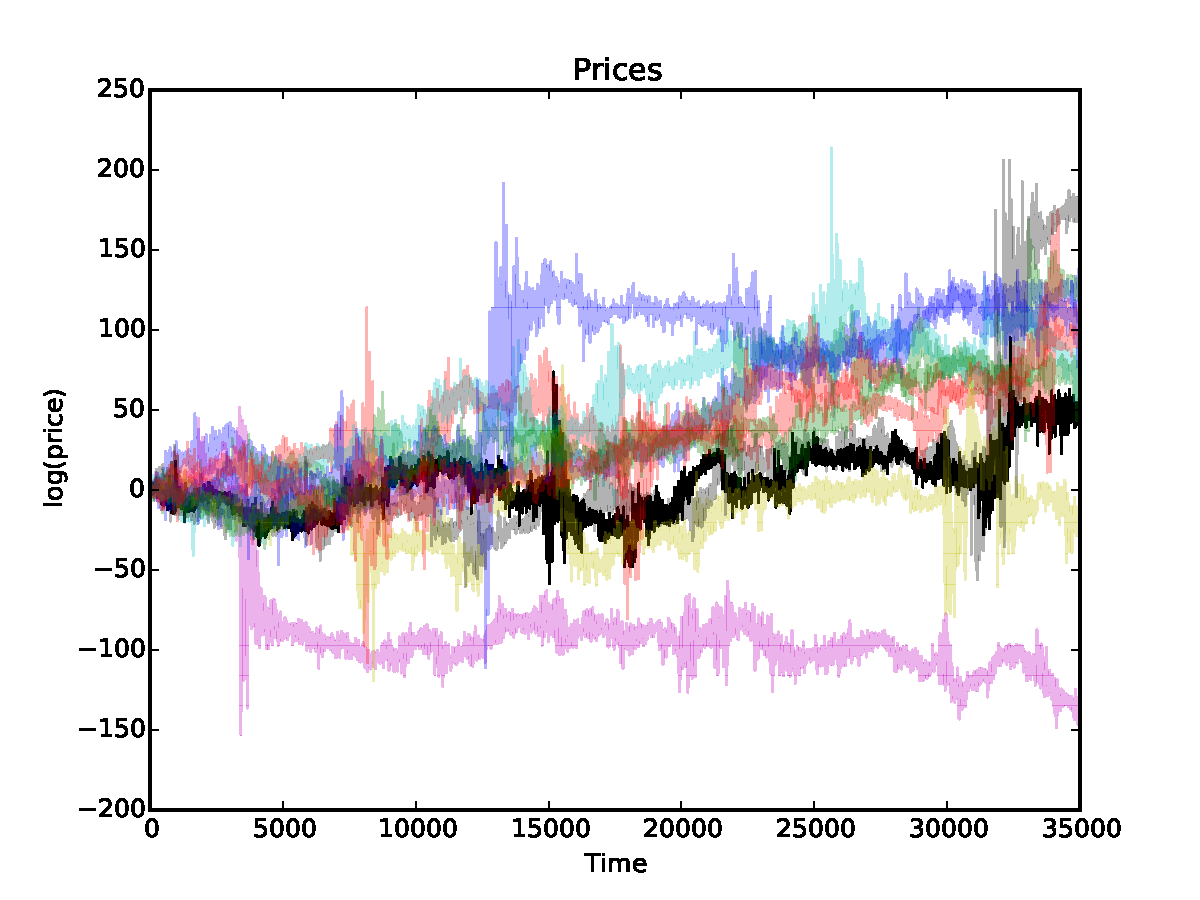
\includegraphics[width=0.5\textwidth]{images/rainbow_ensemble.pdf}
  \caption{Price series from a 10-member ensemble using the same fundamental prices and traders.}
  \label{fig:rainbow}
  \vspace{-40pt}
\end{wrapfigure}

\section{Time series of the system}

The 35000 period-long price series from a 10-member ensemble can be seen in Figure \ref{fig:rainbow}, each displayed in a separate color. The ensemble members all use the same fundamental price series and the same collection of traders, and all start from the same price.
The clustered volatility can be seen best in the blue and black price series. There are intervals of high volatility in the black series near $t=15000$ and $t=32000$, while the rest of this series is relatively nonvolatile. Similarly, the blue series exhibits a long stretch of high volatility between $t=12000$ and $t=15000$ but is less volatile elswhere.

A separate price series generated by the system is displayed in Figure \ref{fig:seriesA}, along with the corresponding returns series. Intervals of high volatility in the market price, such as those near $t=2000$ and $t=20000$, can be seen more clearly in the time series of returns, which indicates roughly four intervals of high volatility.
\begin{figure}[h]
  \centering
  \begin{subfigure}[b]{0.48\textwidth}
    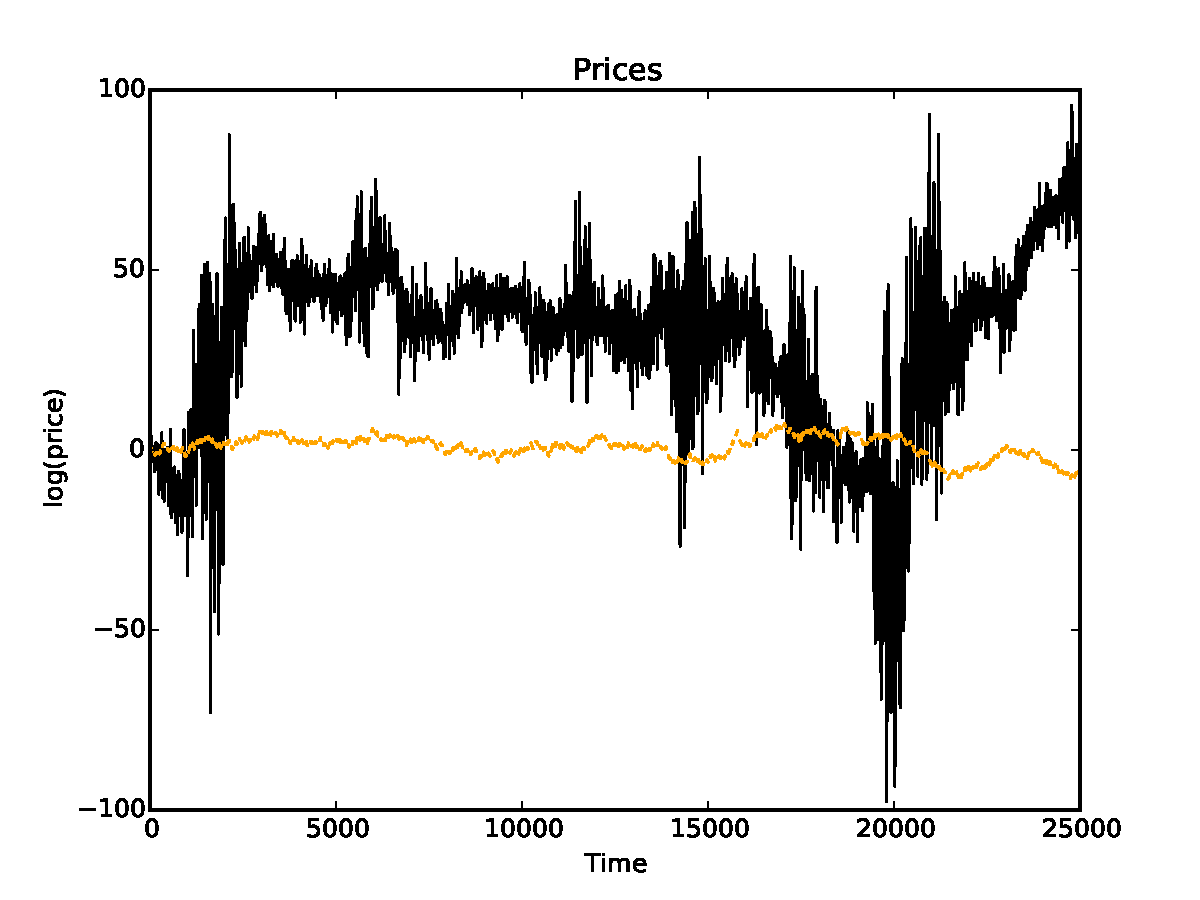
\includegraphics[width=\textwidth]{images/seriesA_prices.pdf}
    \caption{Price series in black. Fundamental prices in orange.}
  \end{subfigure}
  ~
  \begin{subfigure}[b]{0.48\textwidth}
    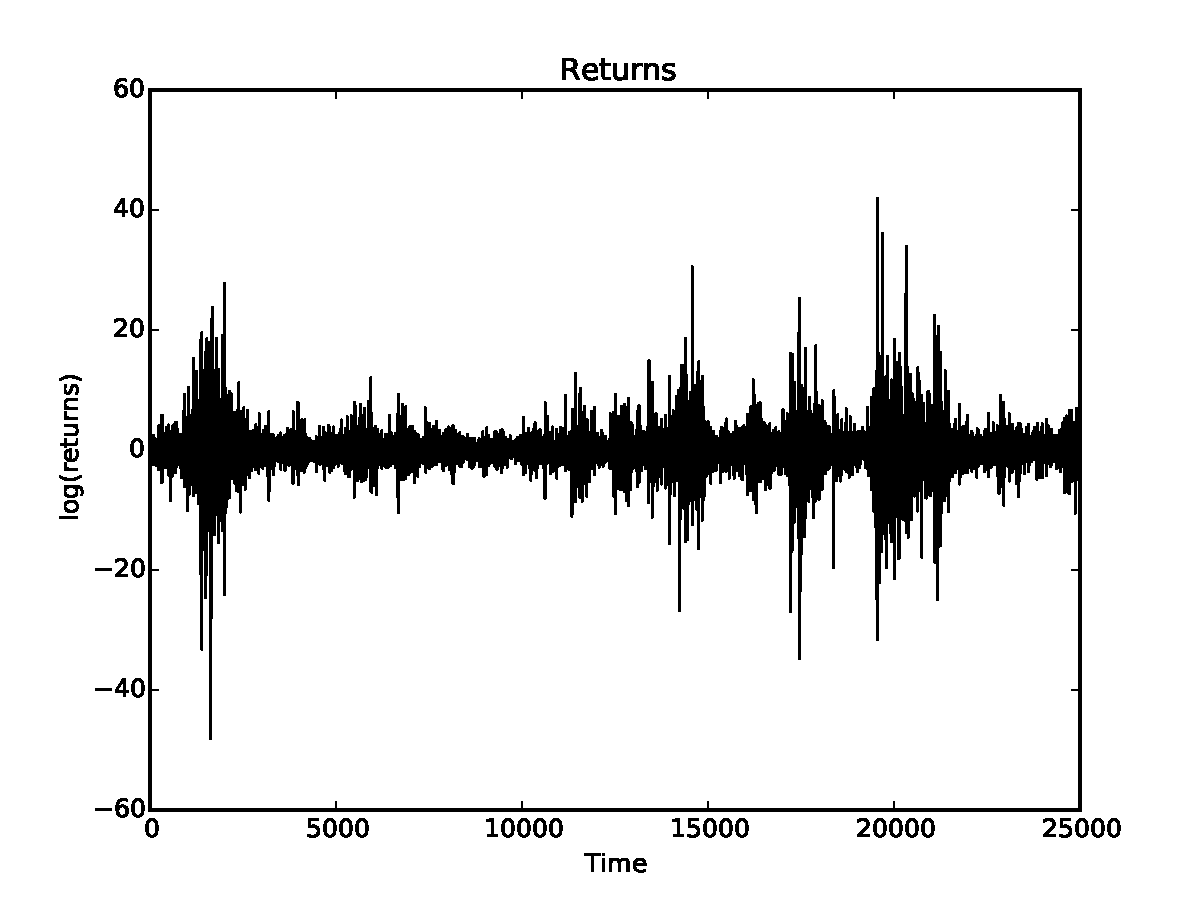
\includegraphics[width=\textwidth]{images/seriesA_returns.pdf}
    \caption{Returns series displaying four volatility clusters.}
  \end{subfigure}
  \caption{Price series and the corresponding returns series.}
  \label{fig:seriesA}
\end{figure}

Plotting the returns of the same series in a histogram, Figure \ref{fig:seriesA_hist}, shows clear leptokurtosis when compared to a Gaussian distribution. These plots confirm Carvalho's and Farmer's observations of leptokurtosis and clustered volatility in this system of heterogeneous agents.

\begin{wrapfigure}{r}{0.5\textwidth}
  \centering
  \vspace{-40pt}
  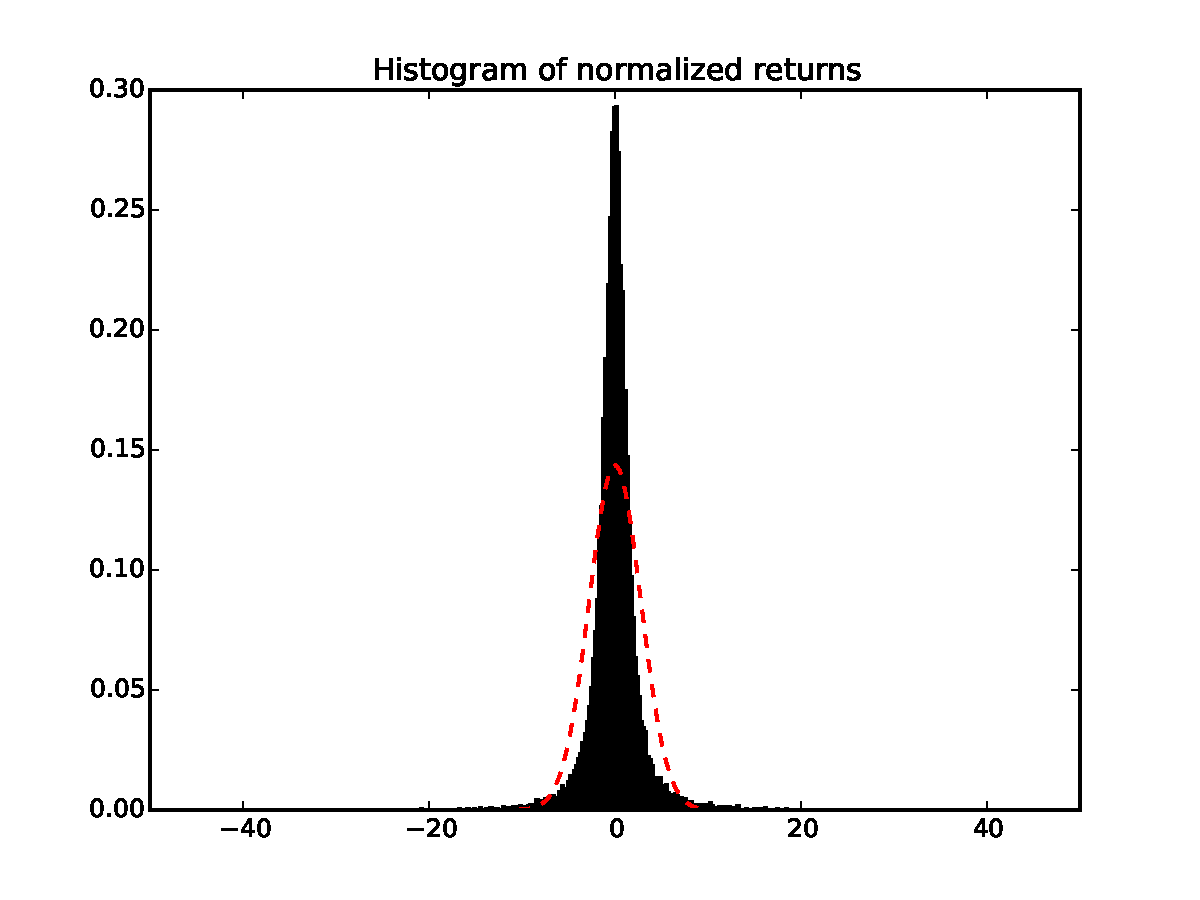
\includegraphics[width=0.5\textwidth]{images/seriesA_histogram.pdf}
  \caption{Returns of the same series as in Figure \ref{fig:seriesA}. Note the sharp peak and fat tails relative to a fitted Gaussian distribution shown as a red dashed line.}
  \label{fig:seriesA_hist}
\end{wrapfigure}

\section{Decay of information}

%N_ens=64
Ensembles such as that in Figure \ref{fig:rainbow} can be used to describe the decay of information of a system as the ensemble tends toward a background distribution. I.e., if we select one price series as the ``true'' price series, then the empirical distribution of the ensemble at a given point in time can be informative about the true price at that time. However, if the distribution of the ensemble is indistinguishable from the background distribution, then the true price is too far in the future to predict.

The background distribution can be estimated by taking the last $\tau$ periods of a simulation and dividing the prices of all ensemble members during those $\tau$ periods into equally sized bins. Suppose there are $N_{bins}$ bins. Then the probability of landing in a given bin is $q=\frac{1}{N_{bins}}$. The estimated background distribution is thus completely described by the edges of the bins. Given an ensemble of size $N_{ens}$, the relative entropy of the ensemble at time $t$ with respect to the background distribution can be computed as follows: Let $n_i$ be the number of ensemble members at time $t$ that fall in the $i$th bin and let $p_i=\frac{n_i}{N_{ens}}$. Then the relative entropy is
$$\mathrm{RE}=\sum_{\substack{1\le i\le N_{ens}\\p_i>0}}p_i\log\frac{p_i}{q}.$$
Note that when $p_i=q$ for all $i$, i.e., the empirical distribution of the ensemble is identical to the estimated background distribution, the relative entropy is zero. Hence an ensemble that has tended toward the background distribution is uninformative.

\begin{wrapfigure}{r}{0.5\textwidth}
  \centering
  \includegraphics[width=0.5\textwidth]{images/entropy.pdf}
  \caption{Relative entropy of this particular ensemble decays rapidly in the first 5000 periods and then more slowly for the rest.}
  \label{fig:entropy}
  \vspace{-20pt}
\end{wrapfigure}
The above analysis has been implemented with $\tau=5000$, $N_{ens}=64$, and $N_{bins}=20$ for a particular realization of the model. The relative entropy at each period is plotted in Figure \ref{fig:entropy}. Note that most of the information is lost in the first 5000 periods. After $t=15000$, the relative entropy is close to zero.

One can see the ensemble tend toward the background distribution by plotting the ensemble along with the true price series. Rather than plotting the price series of every ensemble member as in Figure \ref{fig:rainbow}, the ensemble is summarized in Figure \ref{fig:isopleths} by shading the region between the 1\% isoleth and 99\% isopleth in light green, shading the region between the 10\% isopleth and the 90\% isopleth in slightly darker green, etc. After $t=15000$, the distribution of the ensemble appears similar to the distribution in the last $\tau=5000$ periods, which reflects the relative entropy being close to zero after $t=15000$.

\begin{figure}[h]
  \centering
  \includegraphics[width=0.8\textwidth]{images/isopleths.pdf}
  \caption{True price series is black. Fundamental price series is purple. The $1\%, 10\%, 20\%, \ldots, 80\%, 90\%, 99\%$ isopleths of the ensemble are shaded in increasingly dark green. The ensemble appears close to the background distribution by $t=15000$.}
  \label{fig:isopleths}
\end{figure}

\section{Prediction with an alternative system}

The system can be modified in a variety of ways. Parameters such as the total number of traders, the ratio of fundamentalists to chartists, the distribution of capital among traders, and the distribution of lags that interest the traders can all be tweaked. The model can also be structurally modified by changing the trading strategies or creating a more diverse pool of strategies, incorporating more complicated trend-following techniques. Additionally, traders can be designed to learn from other traders and adopt their strategies depending on their success.

Beyond testing how robust the leptokurtosis and clustered volatility of Carvalho's and Farmer's model is to changes in the parameters and structure, one can also use the alternative systems as models to try to predict the original system.
This could be achieved as follows
\begin{enumerate}
\item Construct a price series from the original system and call it the true price series.
\item Run a large ensemble using the alternative system.
\item Use kernel density estimation to derive a probability density function from the ensemble. (Scoring different bandwidths would help select an ideal bandwidth for the kernel.)
\item Compute the ignorance score of the probability density function at each period given the true price at that period.
\end{enumerate}
This procedure will produce a plot of the ignorance score versus time, showing how the predictability of the original system using the alternative system varies with time. One can also do the converse, i.e., use the same procedure but select the alternative system as truth and use the original system for prediction.

Although the above procedure has not been implemented for this paper, other analysis suggests that the original system is not robust to changes in the fundamentalist trading strategy. As noted above, fundamentalists in Farmer's and Carvalho's models are indifferent to the gap between market price and fundamental price, which does not reflect fundamentalist strategies that are taught in business schools and believed by amateur investors. The unbounded positions that Farmer postulates are bounded by the trader's budget or portfolio size.

Changing the model so that the fundamentalists' strategy is linear in the gap between market and fundamental prices, i.e.,
$$
\omega_{t+1}^{(i)}=c^{(i)}(v_t-p_t),
$$
shatters what turns out to be a delicate balance between fundamentalists and chartists. The price oscillates with unboundedly increasing amplitude, confirming Farmer's postulation. When the fundamentalists orders are bounded by a function of the form of $1-e^{-x}$, the chartists drive the price to $\pm\infty$. When all orders are bounded through this functional form, the price series does not explode, but it no longer exhibits leptokurtosis or clustered volatility. Figure \ref{fig:broken} shows one short realization of this modified system.
\begin{figure}[h]
  \centering
  \begin{subfigure}[b]{0.48\textwidth}
    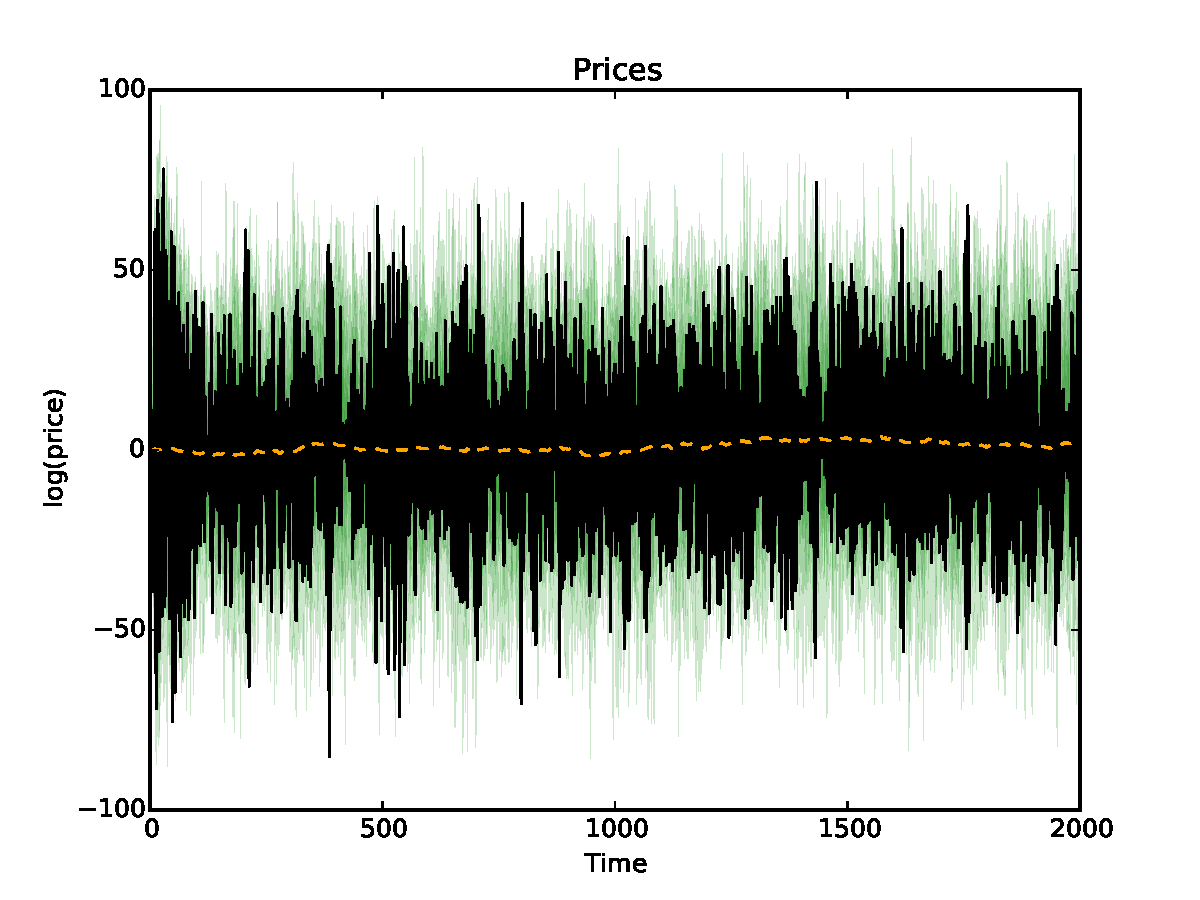
\includegraphics[width=\textwidth]{images/broken_prices.pdf}
    \caption{Price series shown in black. Fundamental prices in orange.}
  \end{subfigure}
  ~
  \begin{subfigure}[b]{0.48\textwidth}
    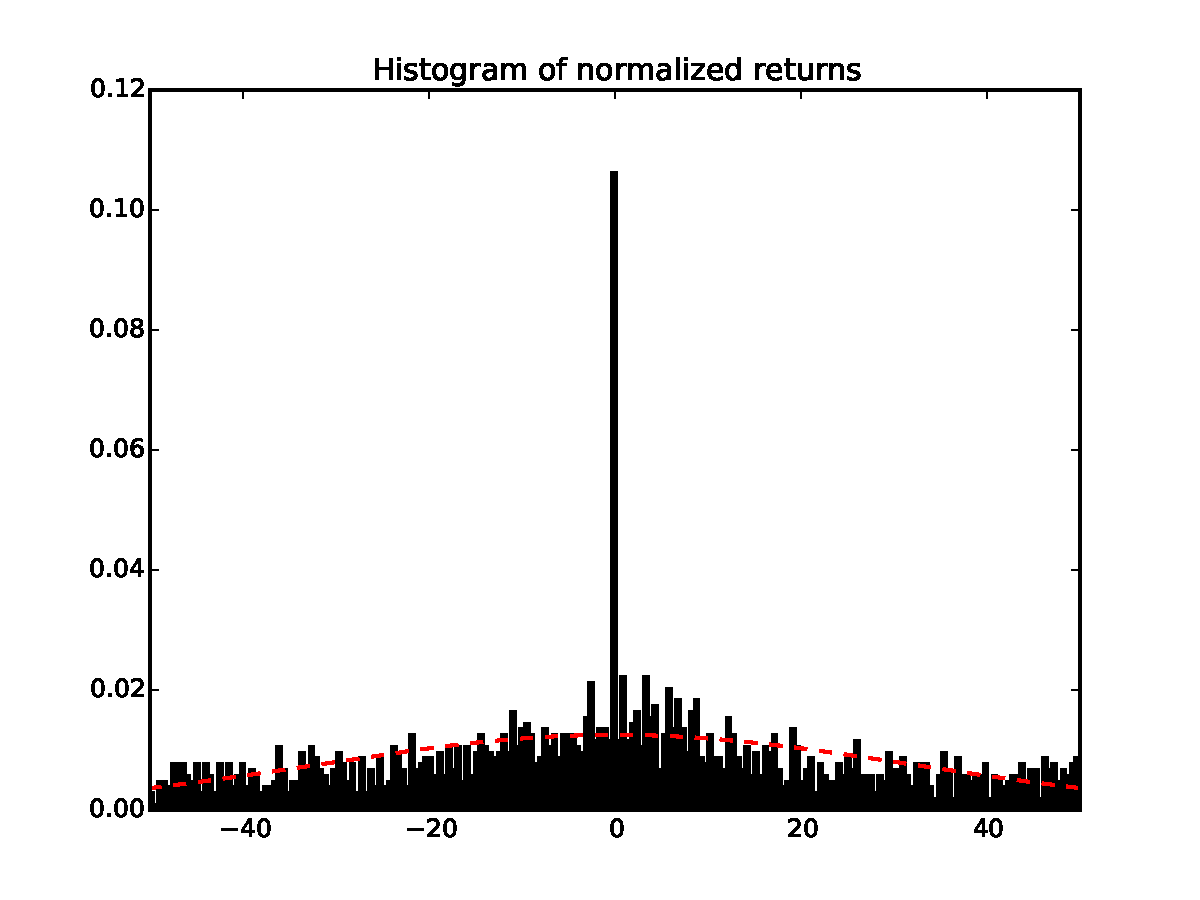
\includegraphics[width=\textwidth]{images/broken_hist.pdf}
    \caption{Returns shown in black with fitted Gaussian distribution in red.}
  \end{subfigure}
  \caption{When fundamentalists trade based on the difference between market and fundamental prices and when all orders are bounded, the system lacks leptokurtosis and clustered volatility.}
  \label{fig:broken}
\end{figure}
This brief analysis suggests that leptokurtosis and clustered volatility found in financial markets in which traders are interested in the level of the fundamental price, rather than just its first derivative, must be caused by structure not included in Carvalho's and Farmer's models.

\section{Interesting insights}

Exploring the modified model above, in which fundamentalists trade linearly in the difference between market and fundamental prices, suggests that the original system is fragile. This can be exploited to better predict the true system. Knowing which modifications of the parameters and the structure shatter the delicate balance achieved in Carvalho's model can narrow down the space of possible structures and parameters that the true system lies in. Indeed, it is even possible that certain structual modifications produce signals in the price or returns series, which would further restrict the set of possible structures.

Relative entropy plots can be used to gauge how far into the future one can predict. Suppose that an ensemble started today reaches the background distribution in 5000 periods. Then knowledge of the history of the price series before today does not help one predict the price at $t=7000$. One should instead predict based on the background distribution. However, the time it takes for the ensemble to reach the background distribution could vary depending on the price or volatility today, which would indicate that some days allow one to predict further into the future than other days. (This variation in predictability was not explored for this paper since the simulation requires a significant amount of CPU time to run for long intervals.)


\begin{thebibliography}{9}

\bibitem{carvalho}
Carvalho, Rui.
``The Dynamics of the Linear Random Farmer Model''
\textit{arXiv}.
(July 2001).
\url{http://arxiv.org/pdf/cond-mat/0107150v1.pdf}

\bibitem{farmer}
Farmer, J. Doyne.
``Market force, ecology and evolution.''
\textit{Industrial and Corporate Change}.
Vol. 11, No. 5 (1998),
pp. 895--953.

\end{thebibliography}

\bibliographystyle{plainnat}

\end{document}


